%%%%%%%%%%%%  Generated using docx2latex.com  %%%%%%%%%%%%%%

%%%%%%%%%%%%  v2.0.0-beta  %%%%%%%%%%%%%%

\documentclass[12pt]{article}
\usepackage{amsmath}
\usepackage{latexsym}
\usepackage{amsfonts}
\usepackage[normalem]{ulem}
\usepackage{soul}
\usepackage{array}
\usepackage{amssymb}
\usepackage{extarrows}
\usepackage{graphicx}
\usepackage[backend=biber,
style=numeric,
sorting=none,
isbn=false,
doi=false,
url=false,
]{biblatex}\addbibresource{bibliography.bib}

\usepackage{subfig}
\usepackage{wrapfig}
\usepackage{wasysym}
\usepackage{enumitem}
\usepackage{adjustbox}
\usepackage{ragged2e}
\usepackage[svgnames,table]{xcolor}
\usepackage{tikz}
\usepackage{longtable}
\usepackage{changepage}
\usepackage{setspace}
\usepackage{hhline}
\usepackage{multicol}
\usepackage{tabto}
\usepackage{float}
\usepackage{multirow}
\usepackage{makecell}
\usepackage{fancyhdr}
\usepackage[toc,page]{appendix}
\usepackage[hidelinks]{hyperref}
\usetikzlibrary{shapes.symbols,shapes.geometric,shadows,arrows.meta}
\tikzset{>={Latex[width=1.5mm,length=2mm]}}
\usepackage{flowchart}\usepackage[paperheight=11.69in,paperwidth=8.27in,left=1.0in,right=1.0in,top=1.0in,bottom=1.0in,headheight=1in]{geometry}
\usepackage[utf8]{inputenc}
\usepackage[T1]{fontenc}
\TabPositions{0.5in,1.0in,1.5in,2.0in,2.5in,3.0in,3.5in,4.0in,4.5in,5.0in,5.5in,6.0in,}

\urlstyle{same}

\renewcommand{\_}{\kern-1.5pt\textunderscore\kern-1.5pt}

 %%%%%%%%%%%%  Set Depths for Sections  %%%%%%%%%%%%%%

% 1) Section
% 1.1) SubSection
% 1.1.1) SubSubSection
% 1.1.1.1) Paragraph
% 1.1.1.1.1) Subparagraph


\setcounter{tocdepth}{5}
\setcounter{secnumdepth}{5}


 %%%%%%%%%%%%  Set Depths for Nested Lists created by \begin{enumerate}  %%%%%%%%%%%%%%


\setlistdepth{9}
\renewlist{enumerate}{enumerate}{9}
		\setlist[enumerate,1]{label=\arabic*)}
		\setlist[enumerate,2]{label=\alph*)}
		\setlist[enumerate,3]{label=(\roman*)}
		\setlist[enumerate,4]{label=(\arabic*)}
		\setlist[enumerate,5]{label=(\Alph*)}
		\setlist[enumerate,6]{label=(\Roman*)}
		\setlist[enumerate,7]{label=\arabic*}
		\setlist[enumerate,8]{label=\alph*}
		\setlist[enumerate,9]{label=\roman*}

\renewlist{itemize}{itemize}{9}
		\setlist[itemize]{label=$\cdot$}
		\setlist[itemize,1]{label=\textbullet}
		\setlist[itemize,2]{label=$\circ$}
		\setlist[itemize,3]{label=$\ast$}
		\setlist[itemize,4]{label=$\dagger$}
		\setlist[itemize,5]{label=$\triangleright$}
		\setlist[itemize,6]{label=$\bigstar$}
		\setlist[itemize,7]{label=$\blacklozenge$}
		\setlist[itemize,8]{label=$\prime$}

\setlength{\topsep}{0pt}\setlength{\parindent}{0pt}

 %%%%%%%%%%%%  This sets linespacing (verticle gap between Lines) Default=1 %%%%%%%%%%%%%%


\renewcommand{\arraystretch}{1.3}

\title{SNA Fall 19 Retake}
\date{}


%%%%%%%%%%%%%%%%%%%% Document code starts here %%%%%%%%%%%%%%%%%%%%



\begin{document}

\maketitle
\par

\chapter{Service description}\par

\begin{FlushRight}
\tab \tab \tab \tab \tab \tab Made by:
\end{FlushRight}\par

\begin{FlushRight}
Ramil Askarov
\end{FlushRight}\par


\vspace{\baselineskip}

\vspace{\baselineskip}
\begin{FlushLeft}
\textbf{Task:}
\end{FlushLeft}\par

\begin{adjustwidth}{0.5in}{0.0in}
\begin{FlushLeft}
Implement Docker-based logging service which collect logs from applications container, Nginx and hosts’s system logs using Fluentd
\end{FlushLeft}\par

\end{adjustwidth}


\vspace{\baselineskip}
\begin{enumerate}
	\item \textbf{System overview}\par

\tab 
\vspace{\baselineskip}\begin{FlushLeft}
\tab All required services starts from docker-compose:
\end{FlushLeft}\par


\vspace{\baselineskip}
\begin{FlushLeft}
\tab \textbf{Fluentd} - Daemon that collects logs from applications and host
\end{FlushLeft}\par

\begin{FlushLeft}
\tab \textbf{Influxdb} - Data storage for our logs
\end{FlushLeft}\par

\begin{FlushLeft}
\tab \textbf{Chronograf} - GUI for Influxdb
\end{FlushLeft}\par

\begin{FlushLeft}
\tab \textbf{Nginx} - Reverse proxy for all System
\end{FlushLeft}\par

\begin{FlushLeft}
\tab \textbf{Web} - Simple flask app 
\end{FlushLeft}\par


\vspace{\baselineskip}

\vspace{\baselineskip}

\vspace{\baselineskip}

\vspace{\baselineskip}
\tab 
\vspace{\baselineskip}
\vspace{\baselineskip}

\vspace{\baselineskip}
\begin{FlushLeft}
System network diagram:
\end{FlushLeft}\par



%%%%%%%%%%%%%%%%%%%% Figure/Image No: 1 starts here %%%%%%%%%%%%%%%%%%%%

\begin{figure}[H]
	\begin{FlushLeft}		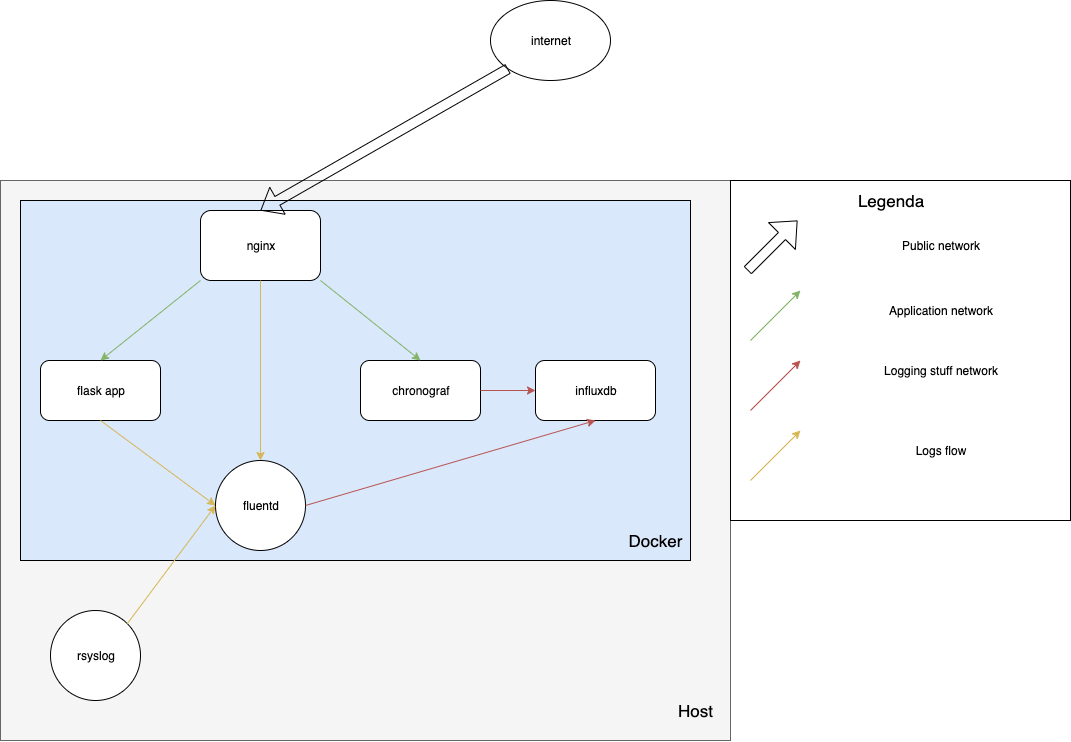
\includegraphics[width=4.78in,height=3.31in]{./media/image1.png}
	\end{FlushLeft}\end{figure}


%%%%%%%%%%%%%%%%%%%% Figure/Image No: 1 Ends here %%%%%%%%%%%%%%%%%%%%

\tab \par


\vspace{\baselineskip}

\vspace{\baselineskip}

\vspace{\baselineskip}

\vspace{\baselineskip}

\vspace{\baselineskip}

\vspace{\baselineskip}

\vspace{\baselineskip}

\vspace{\baselineskip}

\vspace{\baselineskip}

\vspace{\baselineskip}

\vspace{\baselineskip}

\vspace{\baselineskip}

\vspace{\baselineskip}

\vspace{\baselineskip}

\vspace{\baselineskip}
	\item \textbf{Used docker images}\par

\begin{itemize}
	\item i\textbf{nfluxdb:1.7.4} official Influxdb image, Dockerfile can be found in /influx directory\par

	\item \textbf{fluentd-influxdb:latest }official fluent image with installed plugin for Influxdb, Dockerfile can be found in /fluent directory\par

	\item \textbf{chronograf:latest} official Chronograf image, Dockerfile can be found in /chronograf directory\par

	\item \textbf{nignx:latest }official Nginx image\par

	\item \textbf{rome314/sna-retake-flask:latest }image of my flask application from DockerHub, Dockerfile can be found in /flask directory
\end{itemize}\par


\vspace{\baselineskip}
	\item \textbf{Already implemented/Need to be implemented}\par


\vspace{\baselineskip}
\begin{FlushLeft}
Done:
\end{FlushLeft}\par

\begin{itemize}
	\item Plug-and-play system:
\end{itemize}\par

\begin{adjustwidth}{1.0in}{0.0in}
\begin{FlushLeft}
Only you need for running system is clone repository and run one script
\end{FlushLeft}\par

\end{adjustwidth}

\begin{itemize}
	\item Handling all system logs from host machine\par

	\item Created dashboards for Chronograf which need to import manually 
\end{itemize}\par

\begin{FlushLeft}
\tab TODO:
\end{FlushLeft}\par

\begin{itemize}
	\item Auto-import predefined dashboards to Chronograf:
\end{itemize}\par

\begin{adjustwidth}{1.0in}{0.0in}
\begin{FlushLeft}
I could not import dashboards to Chronograf in automated way
\end{FlushLeft}\par

\end{adjustwidth}

\begin{itemize}
	\item Add graphs and plots to dashboards\par

	\item Parse syslogs by sources, types 
\end{itemize}\par


\vspace{\baselineskip}
\tab 
\vspace{\baselineskip}\tab 
\vspace{\baselineskip}	\item \textbf{Used to Test:}
\end{enumerate}\par

\begin{itemize}
	\item AWS t2.micro instance\par

	\item {\fontsize{11pt}{13.2pt}\selectfont \textcolor[HTML]{444444}{Ubuntu Server 18.04 LTS}\par}\par

	\item {\fontsize{11pt}{13.2pt}\selectfont \textcolor[HTML]{444444}{Docker, docker-compose}\par}\par

	\item {\fontsize{11pt}{13.2pt}\selectfont \textcolor[HTML]{444444}{rsyslog}\par}
\end{itemize}\par


\vspace{\baselineskip}

\vspace{\baselineskip}

\printbibliography
\end{document}